%%%% Paramétrage du TD %%%%
\def\xxactivite{Révisions \ifprof -- Corrigé \else \fi} % \normalsize \vspace{-.4cm}
\def\xxauteur{\textsl{Xavier Pessoles}}


\def\xxnumchapitre{Révision 1 \vspace{.2cm}}
\def\xxchapitre{\hspace{.12cm} Résolution des problèmes de statique -- Statique 2D}
\def\xxonglet{\textsf{Rév -- Stat}}
\def\xxactivite{TD 01}
\def\xxauteur{\textsl{Xavier Pessoles}}

\def\xxpied{%
Révision statique -- Résolution des problèmes de statique plane\\
Fiche 1 -- \xxactivite%
}

\def\xxcompetences{%
\vspace{-.3cm}
\textsl{%
\textbf{Savoirs et compétences :}\\
%\vspace{-.4cm}
%\begin{itemize}[label=\ding{112},font=\color{ocre}] 
%%\item \textit{Res1.C4 : } Correction
% \item \textit{Res1.C4.SF1 : } Proposer la démarche de réglage d’un correcteur proportionnel
%%proportionnel intégral 
%%et à avance de phase
%\item \textit{Con.C2 : } 	Correction d’un système asservi	
%\item \textit{Con.C2.SF1 : } Choisir un type de correcteur adapté
%\end{itemize}
}}

\def\xxauteur{\textsl{Xavier Pessoles}}

\def\xxtitreexo{Modélisation d'un hayon de coffre électrique}
\def\xxsourceexo{\hspace{.2cm} \footnotesize{Concours Centrale Supelec TSI 2013}}

\def\xxfigures{
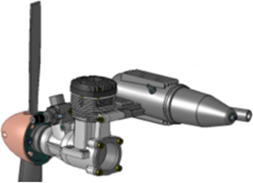
\includegraphics[width=.55\textwidth]{fig_00}
}%figues de la page de garde


\iflivret
\pagestyle{empty}


%%%%%%%% PAGE DE GARDE COURS
\ifcours
% ==== BANDEAU DES TITRES ==== 
\begin{tikzpicture}[remember picture,overlay]
\node at (current page.north west)
{\begin{tikzpicture}[remember picture,overlay]
\node[anchor=north west,inner sep=0pt] at (0,0) {\includegraphics[width=\paperwidth]{\thechapterimage}};
\draw[anchor=west] (-2cm,-8cm) node [line width=2pt,rounded corners=15pt,draw=ocre,fill=white,fill opacity=0.6,inner sep=40pt]{\strut\makebox[22cm]{}};
\draw[anchor=west] (1cm,-8cm) node {\huge\sffamily\bfseries\color{black} %
\begin{minipage}{1cm}
\rotatebox{90}{\LARGE\sffamily\textsc{\color{ocre}\textbf{\xxnumpartie}}}
\end{minipage} \hfill
\begin{minipage}[c]{14cm}
\begin{titrepartie}
\begin{flushright}
\renewcommand{\baselinestretch}{1.1} 
\Large\sffamily\textsc{\textbf{\xxpartie}}
\renewcommand{\baselinestretch}{1} 
\end{flushright}
\end{titrepartie}
\end{minipage} \hfill
\begin{minipage}[c]{3.5cm}
{\large\sffamily\textsc{\textbf{\color{ocre} \discipline}}}
\end{minipage} 
 };
\end{tikzpicture}};
\end{tikzpicture}
% ==== FIN BANDEAU DES TITRES ==== 


% ==== ONGLET 
\begin{tikzpicture}[overlay]
\node[shape=rectangle, 
      rounded corners = .25 cm,
	  draw= ocre,
	  line width=2pt, 
	  fill = ocre!10,
	  minimum width  = 2.5cm,
	  minimum height = 3cm,] at (18.3cm,0) {};
\node at (17.7cm,0) {\rotatebox{90}{\textbf{\Large\color{ocre}{\classe}}}};
%{};
\end{tikzpicture}
% ==== FIN ONGLET 


\vspace{3.5cm}

\begin{tikzpicture}[remember picture,overlay]
\draw[anchor=west] (-2cm,-6cm) node {\huge\sffamily\bfseries\color{black} %
\begin{minipage}{2cm}
\begin{center}
\LARGE\sffamily\textsc{\color{ocre}\textbf{\xxactivite}}
\end{center}
\end{minipage} \hfill
\begin{minipage}[c]{15cm}
\begin{titrechapitre}
\renewcommand{\baselinestretch}{1.1} 
\Large\sffamily\textsc{\textbf{\xxnumchapitre}}

\Large\sffamily\textsc{\textbf{\xxchapitre}}
\vspace{.5cm}

\renewcommand{\baselinestretch}{1} 
\normalsize\normalfont
\xxcompetences
\end{titrechapitre}
\end{minipage}  };
\end{tikzpicture}
\vfill

\begin{flushright}
\begin{minipage}[c]{.3\linewidth}
\begin{center}
\xxfigures
\end{center}
\end{minipage}\hfill
\begin{minipage}[c]{.6\linewidth}
\startcontents
%\printcontents{}{1}{}
\printcontents{}{1}{}
\end{minipage}
\end{flushright}

\begin{tikzpicture}[remember picture,overlay]
\draw[anchor=west] (4.5cm,-.7cm) node {
\begin{minipage}[c]{.2\linewidth}
\begin{flushright}

\includegraphics[width=2cm]{logoCC}
\end{flushright}
\end{minipage}
\begin{minipage}[c]{.2\linewidth}
\textsl{\xxauteur} \\
\textsl{\classe}
\end{minipage}
 };
\end{tikzpicture}

\newpage
\pagestyle{fancy}

%\newpage
%\pagestyle{fancy}

\else
\fi
%% FIN PAGE DE GARDE DES COURS

%%%%%%%% PAGE DE GARDE TD
\iftd
%\begin{tikzpicture}[remember picture,overlay]
%\node at (current page.north west)
%{\begin{tikzpicture}[remember picture,overlay]
%\draw[anchor=west] (-2cm,-3.25cm) node [line width=2pt,rounded corners=15pt,draw=ocre,fill=white,fill opacity=0.6,inner sep=40pt]{\strut\makebox[22cm]{}};
%\draw[anchor=west] (1cm,-3.25cm) node {\huge\sffamily\bfseries\color{black} %
%\begin{minipage}{1cm}
%\rotatebox{90}{\LARGE\sffamily\textsc{\color{ocre}\textbf{\xxnumpartie}}}
%\end{minipage} \hfill
%\begin{minipage}[c]{13.5cm}
%\begin{titrepartie}
%\begin{flushright}
%\renewcommand{\baselinestretch}{1.1} 
%\Large\sffamily\textsc{\textbf{\xxpartie}}
%\renewcommand{\baselinestretch}{1} 
%\end{flushright}
%\end{titrepartie}
%\end{minipage} \hfill
%\begin{minipage}[c]{3.5cm}
%{\large\sffamily\textsc{\textbf{\color{ocre} \discipline}}}
%\end{minipage} 
% };
%\end{tikzpicture}};
%\end{tikzpicture}

%%%%%%%%%% PAGE DE GARDE TD %%%%%%%%%%%%%%%
%\begin{tikzpicture}[overlay]
%\node[shape=rectangle, 
%      rounded corners = .25 cm,
%	  draw= ocre,
%	  line width=2pt, 
%	  fill = ocre!10,
%	  minimum width  = 2.5cm,
%	  minimum height = 2.5cm,] at (18.5cm,0) {};
%\node at (17.7cm,0) {\rotatebox{90}{\textbf{\Large\color{ocre}{\classe}}}};
%%{};
%\end{tikzpicture}

% PARTIE ET CHAPITRE
%\begin{tikzpicture}[remember picture,overlay]
%\draw[anchor=west] (-1cm,-2.1cm) node {\large\sffamily\bfseries\color{black} %
%\begin{minipage}[c]{15cm}
%\begin{flushleft}
%\xxnumchapitre \\
%\xxchapitre
%\end{flushleft}
%\end{minipage}  };
%\end{tikzpicture}

% BANDEAU EXO
\iflivret % SI LIVRET
\begin{tikzpicture}[remember picture,overlay]
\draw[anchor=west] (-2cm,-3.3cm) node {\huge\sffamily\bfseries\color{black} %
\begin{minipage}{5cm}
\begin{center}
\LARGE\sffamily\color{ocre}\textbf{\textsc{\xxactivite}}

\begin{center}
\xxfigures
\end{center}

\end{center}
\end{minipage} \hfill
\begin{minipage}[c]{12cm}
\begin{titrechapitre}
\renewcommand{\baselinestretch}{1.1} 
\large\sffamily\textbf{\textsc{\xxtitreexo}}

\small\sffamily{\textbf{\textit{\color{black!70}\xxsourceexo}}}
\vspace{.5cm}

\renewcommand{\baselinestretch}{1} 
\normalsize\normalfont
\xxcompetences
\end{titrechapitre}
\end{minipage}};
\end{tikzpicture}
\else % ELSE NOT LIVRET
\begin{tikzpicture}[remember picture,overlay]
\draw[anchor=west] (-2cm,-4.5cm) node {\huge\sffamily\bfseries\color{black} %
\begin{minipage}{5cm}
\begin{center}
\LARGE\sffamily\color{ocre}\textbf{\textsc{\xxactivite}}

\begin{center}
\xxfigures
\end{center}

\end{center}
\end{minipage} \hfill
\begin{minipage}[c]{12cm}
\begin{titrechapitre}
\renewcommand{\baselinestretch}{1.1} 
\large\sffamily\textbf{\textsc{\xxtitreexo}}

\small\sffamily{\textbf{\textit{\color{black!70}\xxsourceexo}}}
\vspace{.5cm}

\renewcommand{\baselinestretch}{1} 
\normalsize\normalfont
\xxcompetences
\end{titrechapitre}
\end{minipage}};
\end{tikzpicture}

\fi

\else   % FIN IF TD
\fi


%%%%%%%% PAGE DE GARDE FICHE
\iffiche
\begin{tikzpicture}[remember picture,overlay]
\node at (current page.north west)
{\begin{tikzpicture}[remember picture,overlay]
\draw[anchor=west] (-2cm,-2.25cm) node [line width=2pt,rounded corners=15pt,draw=ocre,fill=white,fill opacity=0.6,inner sep=40pt]{\strut\makebox[22cm]{}};
\draw[anchor=west] (1cm,-2.25cm) node {\huge\sffamily\bfseries\color{black} %
\begin{minipage}{1cm}
\rotatebox{90}{\LARGE\sffamily\textsc{\color{ocre}\textbf{\xxnumpartie}}}
\end{minipage} \hfill
\begin{minipage}[c]{14cm}
\begin{titrepartie}
\begin{flushright}
\renewcommand{\baselinestretch}{1.1} 
\large\sffamily\textsc{\textbf{\xxpartie} \\} 

\vspace{.2cm}

\normalsize\sffamily\textsc{\textbf{\xxnumchapitre -- \xxchapitre}}
\renewcommand{\baselinestretch}{1} 
\end{flushright}
\end{titrepartie}
\end{minipage} \hfill
\begin{minipage}[c]{3.5cm}
{\large\sffamily\textsc{\textbf{\color{ocre} \discipline}}}
\end{minipage} 
 };
\end{tikzpicture}};
\end{tikzpicture}

\iflivret
\begin{tikzpicture}[overlay]
\node[shape=rectangle, 
      rounded corners = .25 cm,
	  draw= ocre,
	  line width=2pt, 
	  fill = ocre!10,
	  minimum width  = 2.5cm,
	  minimum height = 2.5cm,] at (18.5cm,.5cm) {};
\node at (17.9cm,.5cm) {\rotatebox{90}{\textsf{\textbf{\large\color{ocre}{\classe}}}}};
%{};
\end{tikzpicture}
\else
\begin{tikzpicture}[overlay]
\node[shape=rectangle, 
      rounded corners = .25 cm,
	  draw= ocre,
	  line width=2pt, 
	  fill = ocre!10,
	  minimum width  = 2.5cm,
%	  minimum height = 2.5cm,] at (18.5cm,1.1cm) {};
	  minimum height = 2.5cm,] at (18.6cm,0.5cm) {};
\node at (18cm,0.5cm) {\rotatebox{90}{\textsf{\textbf{\large\color{ocre}{\classe}}}}};
%{};
\end{tikzpicture}

\fi

\else
\fi



\else
\pagestyle{empty}


%%%%%%%% PAGE DE GARDE COURS
\ifcours
% ==== BANDEAU DES TITRES ==== 
\begin{tikzpicture}[remember picture,overlay]
\node at (current page.north west)
{\begin{tikzpicture}[remember picture,overlay]
\node[anchor=north west,inner sep=0pt] at (0,0) {\includegraphics[width=\paperwidth]{\thechapterimage}};
\draw[anchor=west] (-2cm,-8cm) node [line width=2pt,rounded corners=15pt,draw=ocre,fill=white,fill opacity=0.6,inner sep=40pt]{\strut\makebox[22cm]{}};
\draw[anchor=west] (1cm,-8cm) node {\huge\sffamily\bfseries\color{black} %
\begin{minipage}{1cm}
\rotatebox{90}{\LARGE\sffamily\textsc{\color{ocre}\textbf{\xxnumpartie}}}
\end{minipage} \hfill
\begin{minipage}[c]{14cm}
\begin{titrepartie}
\begin{flushright}
\renewcommand{\baselinestretch}{1.1} 
\Large\sffamily\textsc{\textbf{\xxpartie}}
\renewcommand{\baselinestretch}{1} 
\end{flushright}
\end{titrepartie}
\end{minipage} \hfill
\begin{minipage}[c]{3.5cm}
{\large\sffamily\textsc{\textbf{\color{ocre} \discipline}}}
\end{minipage} 
 };
\end{tikzpicture}};
\end{tikzpicture}
% ==== FIN BANDEAU DES TITRES ==== 


% ==== ONGLET 
\begin{tikzpicture}[overlay]
\node[shape=rectangle, 
      rounded corners = .25 cm,
	  draw= ocre,
	  line width=2pt, 
	  fill = ocre!10,
	  minimum width  = 2.5cm,
	  minimum height = 3cm,] at (18.3cm,0) {};
\node at (17.7cm,0) {\rotatebox{90}{\textbf{\Large\color{ocre}{\classe}}}};
%{};
\end{tikzpicture}
% ==== FIN ONGLET 


\vspace{3.5cm}

\begin{tikzpicture}[remember picture,overlay]
\draw[anchor=west] (-2cm,-6cm) node {\huge\sffamily\bfseries\color{black} %
\begin{minipage}{2cm}
\begin{center}
\LARGE\sffamily\textsc{\color{ocre}\textbf{\xxactivite}}
\end{center}
\end{minipage} \hfill
\begin{minipage}[c]{15cm}
\begin{titrechapitre}
\renewcommand{\baselinestretch}{1.1} 
\Large\sffamily\textsc{\textbf{\xxnumchapitre}}

\Large\sffamily\textsc{\textbf{\xxchapitre}}
\vspace{.5cm}

\renewcommand{\baselinestretch}{1} 
\normalsize\normalfont
\xxcompetences
\end{titrechapitre}
\end{minipage}  };
\end{tikzpicture}
\vfill

\begin{flushright}
\begin{minipage}[c]{.3\linewidth}
\begin{center}
\xxfigures
\end{center}
\end{minipage}\hfill
\begin{minipage}[c]{.6\linewidth}
\startcontents
%\printcontents{}{1}{}
\printcontents{}{1}{}
\end{minipage}
\end{flushright}

\begin{tikzpicture}[remember picture,overlay]
\draw[anchor=west] (4.5cm,-.7cm) node {
\begin{minipage}[c]{.2\linewidth}
\begin{flushright}

\includegraphics[width=2cm]{logoCC}
\end{flushright}
\end{minipage}
\begin{minipage}[c]{.2\linewidth}
\textsl{\xxauteur} \\
\textsl{\classe}
\end{minipage}
 };
\end{tikzpicture}

\newpage
\pagestyle{fancy}

%\newpage
%\pagestyle{fancy}

\else
\fi
%% FIN PAGE DE GARDE DES COURS

%%%%%%%% PAGE DE GARDE TD
\iftd
%\begin{tikzpicture}[remember picture,overlay]
%\node at (current page.north west)
%{\begin{tikzpicture}[remember picture,overlay]
%\draw[anchor=west] (-2cm,-3.25cm) node [line width=2pt,rounded corners=15pt,draw=ocre,fill=white,fill opacity=0.6,inner sep=40pt]{\strut\makebox[22cm]{}};
%\draw[anchor=west] (1cm,-3.25cm) node {\huge\sffamily\bfseries\color{black} %
%\begin{minipage}{1cm}
%\rotatebox{90}{\LARGE\sffamily\textsc{\color{ocre}\textbf{\xxnumpartie}}}
%\end{minipage} \hfill
%\begin{minipage}[c]{13.5cm}
%\begin{titrepartie}
%\begin{flushright}
%\renewcommand{\baselinestretch}{1.1} 
%\Large\sffamily\textsc{\textbf{\xxpartie}}
%\renewcommand{\baselinestretch}{1} 
%\end{flushright}
%\end{titrepartie}
%\end{minipage} \hfill
%\begin{minipage}[c]{3.5cm}
%{\large\sffamily\textsc{\textbf{\color{ocre} \discipline}}}
%\end{minipage} 
% };
%\end{tikzpicture}};
%\end{tikzpicture}

%%%%%%%%%% PAGE DE GARDE TD %%%%%%%%%%%%%%%
%\begin{tikzpicture}[overlay]
%\node[shape=rectangle, 
%      rounded corners = .25 cm,
%	  draw= ocre,
%	  line width=2pt, 
%	  fill = ocre!10,
%	  minimum width  = 2.5cm,
%	  minimum height = 2.5cm,] at (18.5cm,0) {};
%\node at (17.7cm,0) {\rotatebox{90}{\textbf{\Large\color{ocre}{\classe}}}};
%%{};
%\end{tikzpicture}

% PARTIE ET CHAPITRE
%\begin{tikzpicture}[remember picture,overlay]
%\draw[anchor=west] (-1cm,-2.1cm) node {\large\sffamily\bfseries\color{black} %
%\begin{minipage}[c]{15cm}
%\begin{flushleft}
%\xxnumchapitre \\
%\xxchapitre
%\end{flushleft}
%\end{minipage}  };
%\end{tikzpicture}

% BANDEAU EXO
\iflivret % SI LIVRET
\begin{tikzpicture}[remember picture,overlay]
\draw[anchor=west] (-2cm,-3.3cm) node {\huge\sffamily\bfseries\color{black} %
\begin{minipage}{5cm}
\begin{center}
\LARGE\sffamily\color{ocre}\textbf{\textsc{\xxactivite}}

\begin{center}
\xxfigures
\end{center}

\end{center}
\end{minipage} \hfill
\begin{minipage}[c]{12cm}
\begin{titrechapitre}
\renewcommand{\baselinestretch}{1.1} 
\large\sffamily\textbf{\textsc{\xxtitreexo}}

\small\sffamily{\textbf{\textit{\color{black!70}\xxsourceexo}}}
\vspace{.5cm}

\renewcommand{\baselinestretch}{1} 
\normalsize\normalfont
\xxcompetences
\end{titrechapitre}
\end{minipage}};
\end{tikzpicture}
\else % ELSE NOT LIVRET
\begin{tikzpicture}[remember picture,overlay]
\draw[anchor=west] (-2cm,-4.5cm) node {\huge\sffamily\bfseries\color{black} %
\begin{minipage}{5cm}
\begin{center}
\LARGE\sffamily\color{ocre}\textbf{\textsc{\xxactivite}}

\begin{center}
\xxfigures
\end{center}

\end{center}
\end{minipage} \hfill
\begin{minipage}[c]{12cm}
\begin{titrechapitre}
\renewcommand{\baselinestretch}{1.1} 
\large\sffamily\textbf{\textsc{\xxtitreexo}}

\small\sffamily{\textbf{\textit{\color{black!70}\xxsourceexo}}}
\vspace{.5cm}

\renewcommand{\baselinestretch}{1} 
\normalsize\normalfont
\xxcompetences
\end{titrechapitre}
\end{minipage}};
\end{tikzpicture}

\fi

\else   % FIN IF TD
\fi


%%%%%%%% PAGE DE GARDE FICHE
\iffiche
\begin{tikzpicture}[remember picture,overlay]
\node at (current page.north west)
{\begin{tikzpicture}[remember picture,overlay]
\draw[anchor=west] (-2cm,-2.25cm) node [line width=2pt,rounded corners=15pt,draw=ocre,fill=white,fill opacity=0.6,inner sep=40pt]{\strut\makebox[22cm]{}};
\draw[anchor=west] (1cm,-2.25cm) node {\huge\sffamily\bfseries\color{black} %
\begin{minipage}{1cm}
\rotatebox{90}{\LARGE\sffamily\textsc{\color{ocre}\textbf{\xxnumpartie}}}
\end{minipage} \hfill
\begin{minipage}[c]{14cm}
\begin{titrepartie}
\begin{flushright}
\renewcommand{\baselinestretch}{1.1} 
\large\sffamily\textsc{\textbf{\xxpartie} \\} 

\vspace{.2cm}

\normalsize\sffamily\textsc{\textbf{\xxnumchapitre -- \xxchapitre}}
\renewcommand{\baselinestretch}{1} 
\end{flushright}
\end{titrepartie}
\end{minipage} \hfill
\begin{minipage}[c]{3.5cm}
{\large\sffamily\textsc{\textbf{\color{ocre} \discipline}}}
\end{minipage} 
 };
\end{tikzpicture}};
\end{tikzpicture}

\iflivret
\begin{tikzpicture}[overlay]
\node[shape=rectangle, 
      rounded corners = .25 cm,
	  draw= ocre,
	  line width=2pt, 
	  fill = ocre!10,
	  minimum width  = 2.5cm,
	  minimum height = 2.5cm,] at (18.5cm,.5cm) {};
\node at (17.9cm,.5cm) {\rotatebox{90}{\textsf{\textbf{\large\color{ocre}{\classe}}}}};
%{};
\end{tikzpicture}
\else
\begin{tikzpicture}[overlay]
\node[shape=rectangle, 
      rounded corners = .25 cm,
	  draw= ocre,
	  line width=2pt, 
	  fill = ocre!10,
	  minimum width  = 2.5cm,
%	  minimum height = 2.5cm,] at (18.5cm,1.1cm) {};
	  minimum height = 2.5cm,] at (18.6cm,0.5cm) {};
\node at (18cm,0.5cm) {\rotatebox{90}{\textsf{\textbf{\large\color{ocre}{\classe}}}}};
%{};
\end{tikzpicture}

\fi

\else
\fi



\fi
\setlength{\columnseprule}{.1pt}

\pagestyle{fancy}
\thispagestyle{plain}

\vspace{5cm}

\def\columnseprulecolor{\color{ocre}}
\setlength{\columnseprule}{0.4pt} 

\setcounter{exo}{0}

\ifprof
%\begin{multicols}{2}
\else
\begin{multicols}{2}
\fi
%%%%%%%%%%%%%%%%%%%%%%%%%%%%%%%%%%%%%%%%%%%%%%%%%%


\section*{Mise en situation}
\ifprof
\else
Le PCS (Power Closure System), conçu par Valéo, est un système d’ouverture et de fermeture automatique de
hayon de coffre automobile.
Le système étant symétrique, les deux vérins sont ramenées dans 
le plan d’évolution de la porte de coffre et leur action mécanique s’exerçant sur la porte de coffre est supposée identique.

On donne un diagramme d'exigence partiel du système étudié. 

\begin{center}
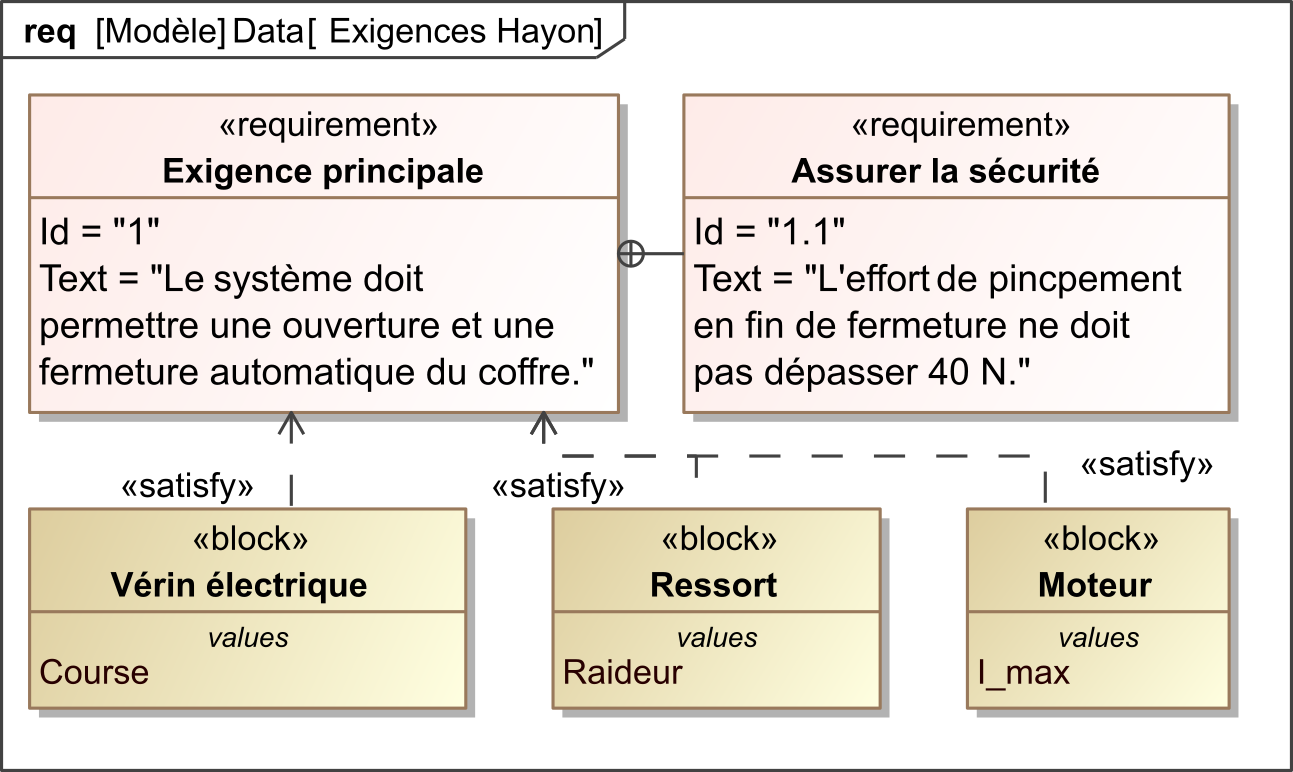
\includegraphics[width=\linewidth]{fig_01_req}
%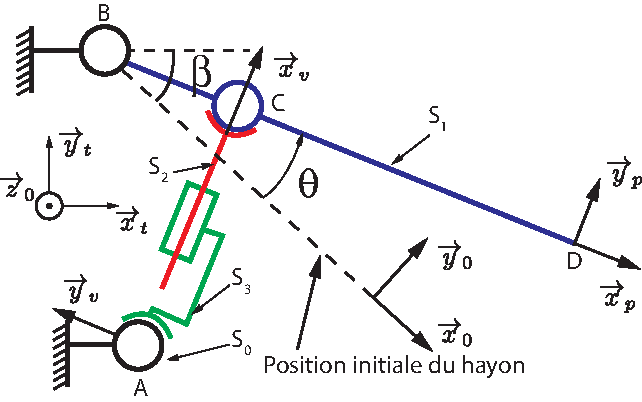
\includegraphics[width=.8\linewidth]{hayon_parametrage}
%\textit{}
\end{center}


\begin{obj}~\\
%\vspace{-.3cm}
\begin{itemize}
\item Déterminer les caractéristiques du vérin répondant au cahier des charges : longueur
du vérin en position coffre ouvert et coffre fermé, course du vérin, raideur du ressort équipant le vérin. 
\item Déterminer le couple moteur maximal nécessaire pour le maintien en position du hayon.
\item Déterminer le courant de pincement afin que l'effort de pincement soit inférieure à \SI{40}{N} pendant \SI{10}{ms}.
\end{itemize}
\end{obj}




Le repère $\repere{B}{x_t}{y_t}{z_0}$ est lié à la Terre. L’accélération de la pesanteur s’écrit $\vect{g}=-g\vect{y_t}$ avec $g=\SI{9,81}{m.s^{-2}}$. La structure du véhicule et la porte de coffre sont en liaison pivot d’axe $\axe{B}{z_0}$.

Le repère $\repere{B}{x_p}{y_p}{z_0}$ est lié à la porte de coffre \textbf{$\bm{S_1}$} de masse $M=\SI{30}{kg}$. Le repère $\repere{B}{x_v}{y_v}{z_0}$ est lié au corps du vérin. La sortie
de tige par rapport au corps du vérin \textbf{$S_3$} se fait dans la direction du vecteur $\vect{x_v}$.
Les liaisons entre le corps du vérin \textbf{$\bm{S_3}$} et le bâti \textbf{$\bm{S_0}$} ainsi qu'entre la tige du vérin \textbf{$\bm{S_2}$} et la porte de coffre \textbf{$\bm{S_1}$} sont des liaisons rotules de centres respectifs $A$ et $C$.
Le point $D$ représente l’extrémité de la porte du coffre. La hauteur du point $D$ par rapport au sol suivant la
verticale est de \SI{0,7}{m} en position coffre fermé et de \SI{1,8}{m} en position coffre ouvert.

%\vspace{-.5cm}

\begin{center}
\includegraphics[width=.8\linewidth]{fig_01_bis}
%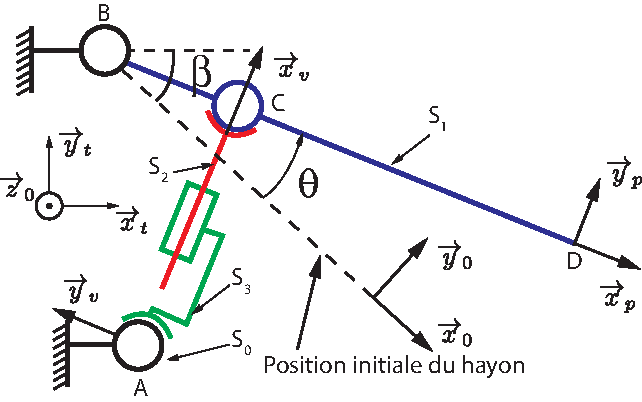
\includegraphics[width=.8\linewidth]{hayon_parametrage}
%\textit{}
\end{center}
\fi

%\vspace{-.5cm}

\subsection*{Caractéristiques géométriques du vérin}
\ifprof
\else
Le centre d’inertie du coffre est situé en $G$ tel que $\vect{BG}=\lambda\vect{x_p}$ avec $\lambda=\SI{0,6}{m}$.

$\vect{AB}=-a\vect{x_0}+b\vect{y_0}$, $\vect{AC}=L\vect{x_v}$, $\vect{BC}=c\vect{x_p}$, $\vect{BD}=d\vect{x_p}$ avec $a=\SI{0,55}{m}$, $b=\SI{0,14}{m}$, $c=\SI{0,14}{m}$  et $d=\SI{1}{m}$. L’angle formé entre $\vect{x_0}$ et l’horizontale $\vect{x_t}$ est $\theta_0 = 42\degres$.
\fi

\subparagraph{}
\textit{Déterminer l’angle d’ouverture maximal.}
\ifprof
\begin{corrige}~\\
\begin{center}
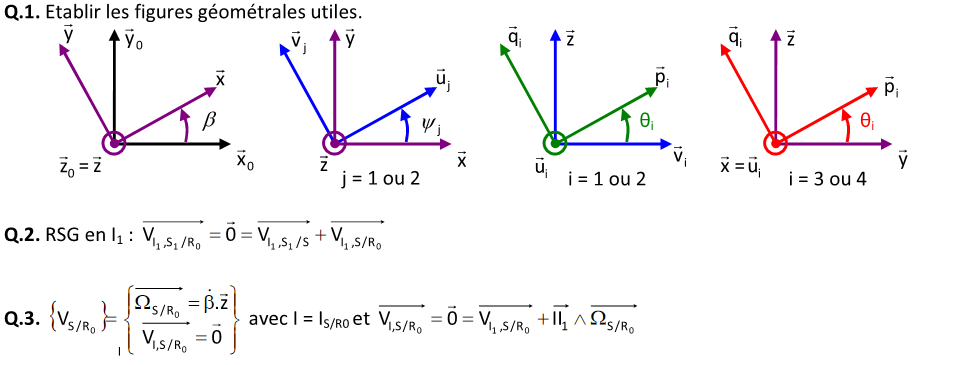
\includegraphics[width=.8\linewidth]{cor_01}
%\textit{}
\end{center}
D'une part, $x = d\sin 42 \simeq \SI{0,67}{m}$. D'autre part, $\sin\alpha = \dfrac{1,8-0,7-x}{d}=0,43$. Au final $\alpha = 25,5\degres$. 

L'angle d'ouverture est donc de $67,5\degres$.

\end{corrige}
\else
\fi

%Par l’écriture de la fermeture géométrique dans le triangle 𝐴𝐵𝐶, déterminer la longueur du vérin 𝐿 en fonction de l’angle d’ouverture du coffre 𝜃.

\subparagraph{}
\textit{Déterminer la longueur du vérin $L$ en fonction de l’angle d’ouverture du coffre $\theta$.}
\ifprof
\begin{corrige}~\\
La longueur du vérin est donnée par la valeur de $L$. En réalisant la fermeture géométrique, on a $\vect{AB}+\vect{BC}+\vect{CA}=\vect{0} \Leftrightarrow 
-a\vect{x_0}+b\vect{y_0} + c\vect{x_p} -L\vect{x_v} =\vect{0}$.

En projetant l'équation vectorielle dans $\rep{0}$, on a : 
$$
\left\{ 
\begin{array}{l}
-a + c\cos\theta -L\cos\alpha ={0} \\
b + c\sin\theta -L\sin\alpha ={0}
\end{array}
\right.
$$
On a donc $L^2 =\left(-a + c\cos\theta \right)^2 + \left(b + c\sin\theta \right)^2  $.
%= a^2 +c^2 \cos ^2 \theta - 2 ac \cos \theta + b^2 + c^2\sin^2\theta + 2b c\sin\theta
%= a^2 +c^2 - 2 ac \cos \theta + b^2 +  2b c\sin\theta$ 

\end{corrige}
\else
\fi

\ifprof
\else
On donne la courbe donnant l'évolution de la course du vérin en fonction de l'ouverture du hayon. 
\begin{center}
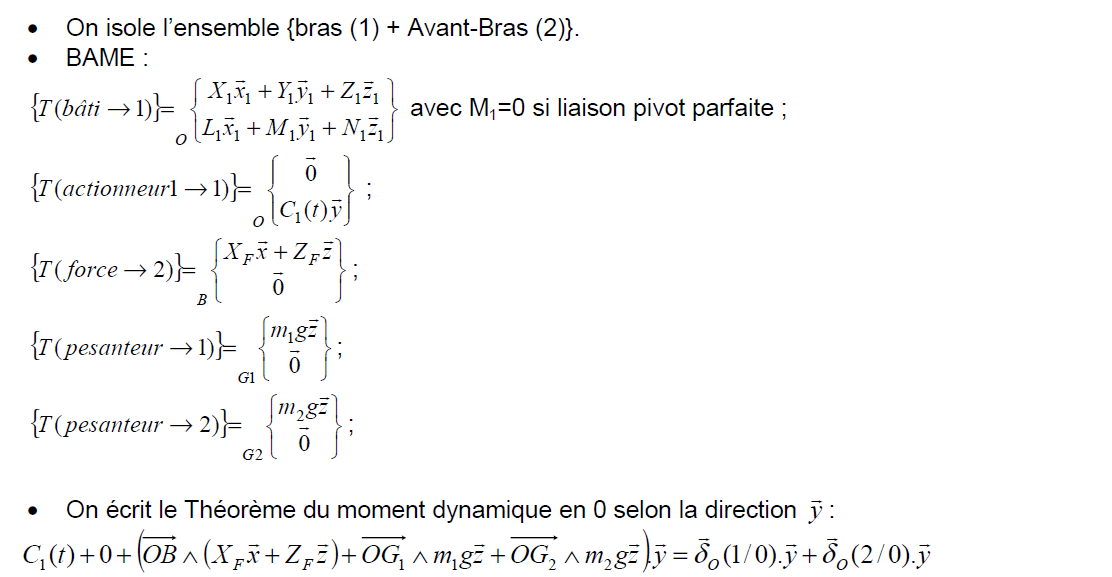
\includegraphics[width=.8\linewidth]{cor_02}
%\textit{}
\end{center}
\fi

%\vspace{-.6cm}

\subparagraph{}
\textit{Déterminer les valeurs extrêmes de $L$, ainsi que la course du vérin.}
\ifprof
\begin{corrige}~\\
La longueur du vérin varie de \SI{43,3}{cm} à \SI{56,5}{cm} soit une course de \SI{13,2}{cm}. 
\end{corrige}
\else
\fi


%
%\vspace{.25cm}
%
%\footnotesize
%\noindent Corrigé des trois premières questions.
%%\fbox{
%\begin{enumerate}
%\item L'angle d'ouverture est de $67,5\degres$.
%\item $L^2 =\left(-a + c\cos\theta \right)^2 + \left(b + c\sin\theta \right)^2  $.
%\item Course de \SI{13,2}{cm}.
%\end{enumerate}
%
%\normalsize
%\fi

\subsection*{Dimensionnement des caractéristiques du ressort}

\ifprof
\else
Les vérins utilisés sont constitués d’un moteur à courant continu, d’un réducteur à engrenage, d’une vis à billes et d’un ressort. Ce dernier permet d'assurer l'équilibre de la porte de coffre en cas de panne des vérins électriques. 

\begin{center}
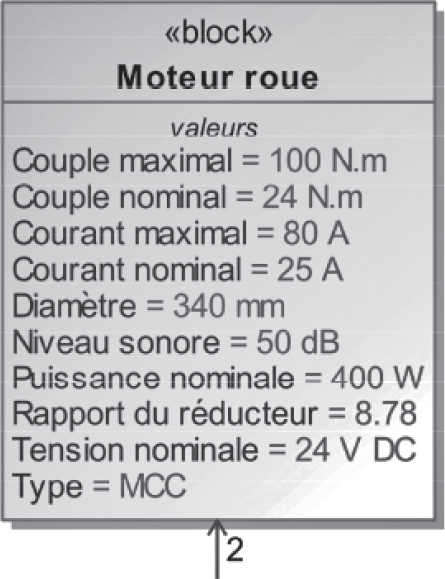
\includegraphics[width=\linewidth]{fig_02}
%\textit{}
\end{center}

%Le cahier des charges impose que la porte soit en équilibre sur une large plage d’ouverture en cas de panne
%moteur. C’est pourquoi il faut déterminer la raideur et la longueur à vide des ressorts qui assurent cette fonction
%dans les vérins électriques.

On suppose dans un premier temps que le coffre est à l’équilibre.
\fi

\subparagraph{}
\textit{Déterminer l’effort $F$ exercé par chacun des vérins sur la porte de coffre en fonction de $\theta$, $\alpha$ et des constantes du problème.}
\ifprof
\begin{corrige}~\\
On isole le corps et le piston du vérin. L'ensemble est soumis à deux actions mécaniques (liaisons sphériques en $A$ et $C$). D'après le PFS, cette action mécanique est donc suivant Ces deux actions mécaniques sont donc de même direction (le vecteur $\vect{x_v}$), de même norme et de sens opposé. 

On isole le hayon $h$. 

On réalise le BAME : 
\begin{itemize}
\item action mécanique du vérin $v$: $\torseurstat{T}{v}{h}=\torseurl{F_v\vect{x_v}}{\vect{0}}{C}$;
\item action de la pesanteur : $\torseurstat{T}{\text{pes}}{h}=\torseurl{-Mg\vect{y_t}}{\vect{0}}{G}$;
\item action de la pivot en $B$ : $\torseurstat{T}{\text{0}}{h}$.
\end{itemize}

On cherche à connaître l'action du vérin en fonction des actions de pesanteur. On réalise donc le théorème du moment statique en $B$ en projection sur $\vect{z_0}$ : 

$ \left( 
\vect{0} + \vect{BC}\wedge F_v\vect{x_v}
+ \vect{0} + \vect{BG}\wedge -Mg\vect{y_t}
\right) \cdot \vect {z_0} = \vect{0} $
$\Rightarrow \left( c\vect{x_p}\wedge F_v\vect{x_v} + \lambda \vect{x_p}\wedge -Mg\vect{y_t}
\right) \cdot \vect {z_0} = \vect{0} $

\begin{center}
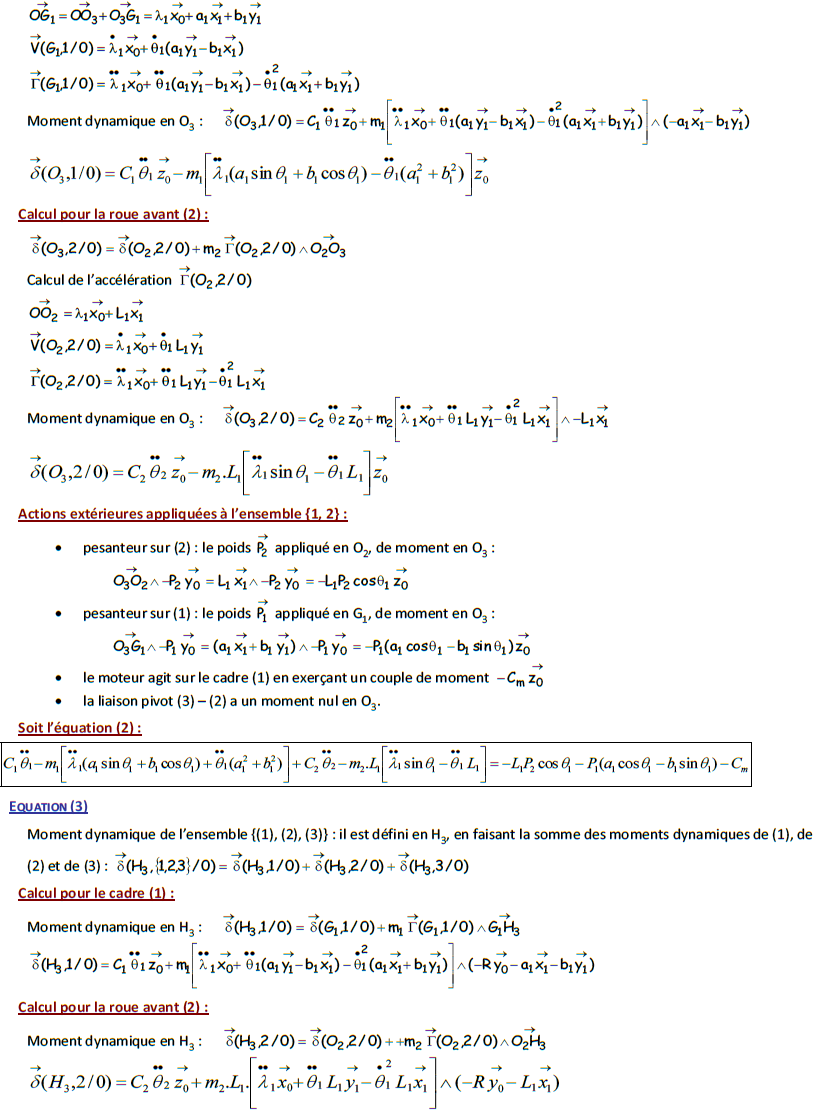
\includegraphics[width=.5\linewidth]{cor_03}
%\textit{}

$\Leftrightarrow  c F_v\sin \left( \alpha - \theta\right) - \lambda Mg\cos \theta  = {0} $

$   F_v = \dfrac{\lambda Mg\cos \theta}{c\sin \left( \alpha - \theta\right)} $.

Dans le cas où on considère les deux vérins, on aura $F_1=F_2=F_v/2$.

\end{center}


\end{corrige}


\else
\fi

\ifprof
\else
En exploitant les équations obtenues à partir de l’écriture de la fermeture géométrique obtenue précédemment, on montre que la relation entre $\theta$ et $\alpha$ s’écrit : 
$ \tan \alpha = \dfrac{b+c\sin\theta}{-a+c\cos\theta}$.

On déduit de la question précédente le tracé de l’évolution de l’effort $F$ nécessaire au maintien en équilibre du coffre en fonction de la longueur $L$ du vérin.


\begin{center}
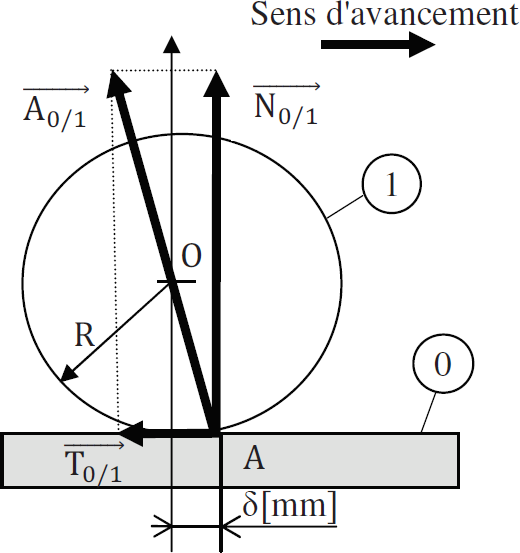
\includegraphics[width=.8\linewidth]{fig_03}
%\textit{}
\end{center}

On choisit d’utiliser un ressort précontraint au sein du vérin de manière à assister l’ouverture du coffre et à assurer l’équilibre du coffre sur une plage de fonctionnement maximale. On estime que les forces de frottement maximales au sein du vérin (essentiellement dues à la friction dans la vis) sont de l’ordre de $F_{\text{frot}}=\SI{100}{N}$. 

La figure précédente représente la force que doit exercer le vérin sur la porte de coffre pour assurer l’équilibre de cette dernière en fonction de la longueur du vérin. Les courbes en pointillés représentent la force du vérin $\pm\SI{100}{N}$.
\fi




\subparagraph{}
\textit{Déterminer la raideur $k$ du ressort et sa longueur à vide $L_0$ de manière à obtenir une situation d’équilibre
sur la plus grande plage de fonctionnement. Préciser votre démarche.}
\ifprof
\begin{corrige}~\\

\begin{center}
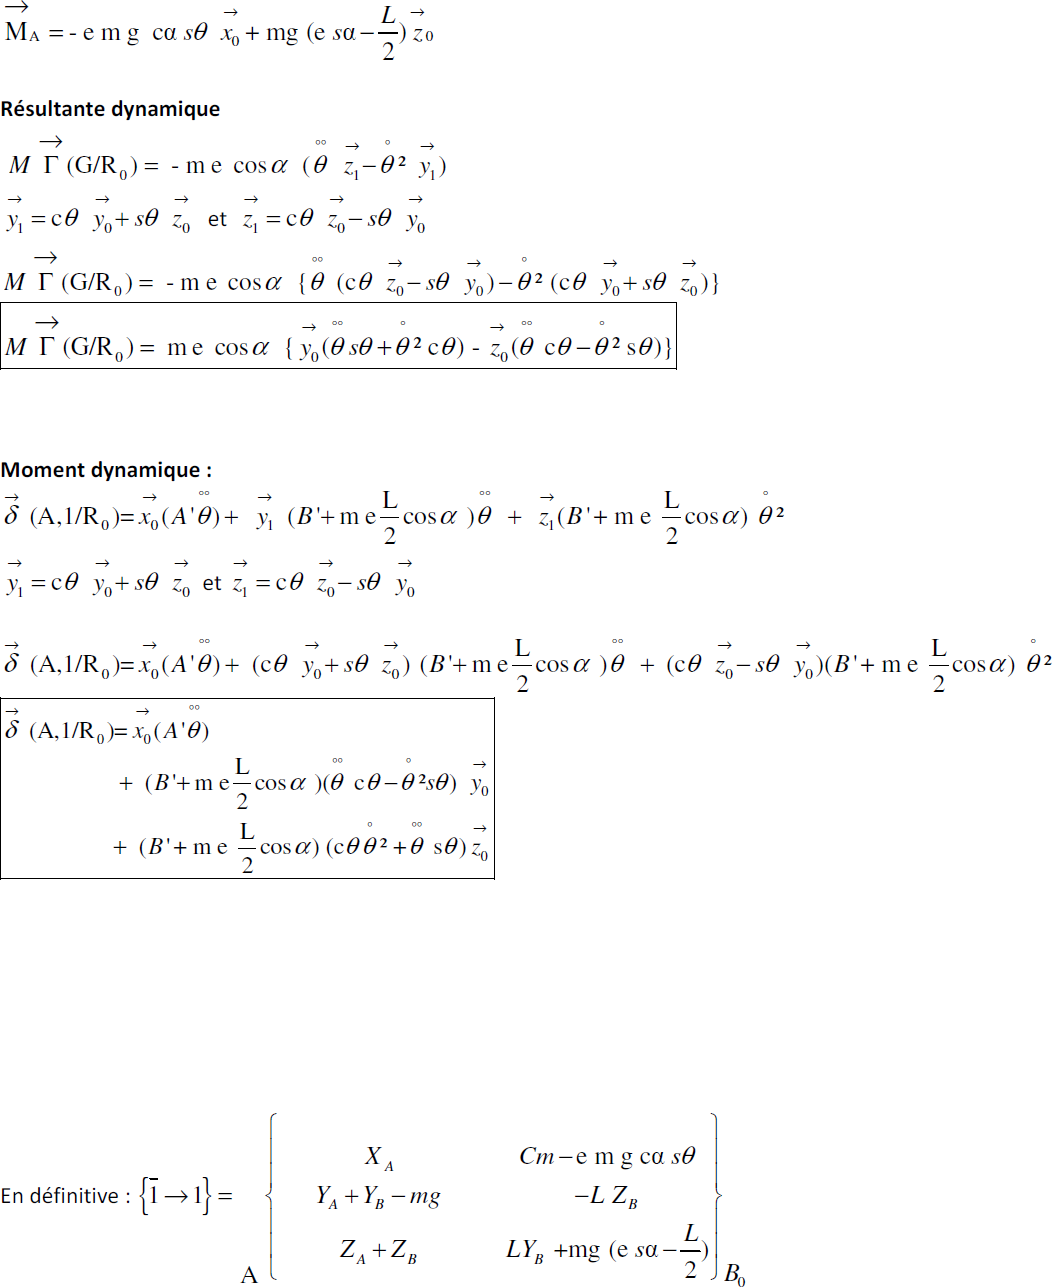
\includegraphics[width=\linewidth]{cor_04}
%\textit{}
\end{center}

Si on isole la tige du vérin :
\begin{itemize}
\item en phase d'ouverture, le TRS s'exprime par : $F_m + F_r - F_f - F_h =0\Leftrightarrow F_r = F_f + F_h - F_m$; 
\item en phase de fermeture, le TRS s'exprime par : $-F_m + F_r + F_f - F_h =0 \Leftrightarrow F_r = -F_f + F_h + F_m$;
\end{itemize}





La plage de fonctionnement la plus large est située entre $\SI{0,5}{m}$ et $\SI{0,56}{m}$. La pente est la même pour les 3 courbes. Elle est d'environ $k=\dfrac{100}{0,06}\simeq \SI{1667}{N.m^{-1}}$.

En phase de fermeture, lorsque le vérin est déployé, la précharge permettant d'assurer l'équilibre est d'environ \SI{500}{N}.  L'écrasement est donc  de \SI{300}{mm} environ.

\end{corrige}
\begin{center}
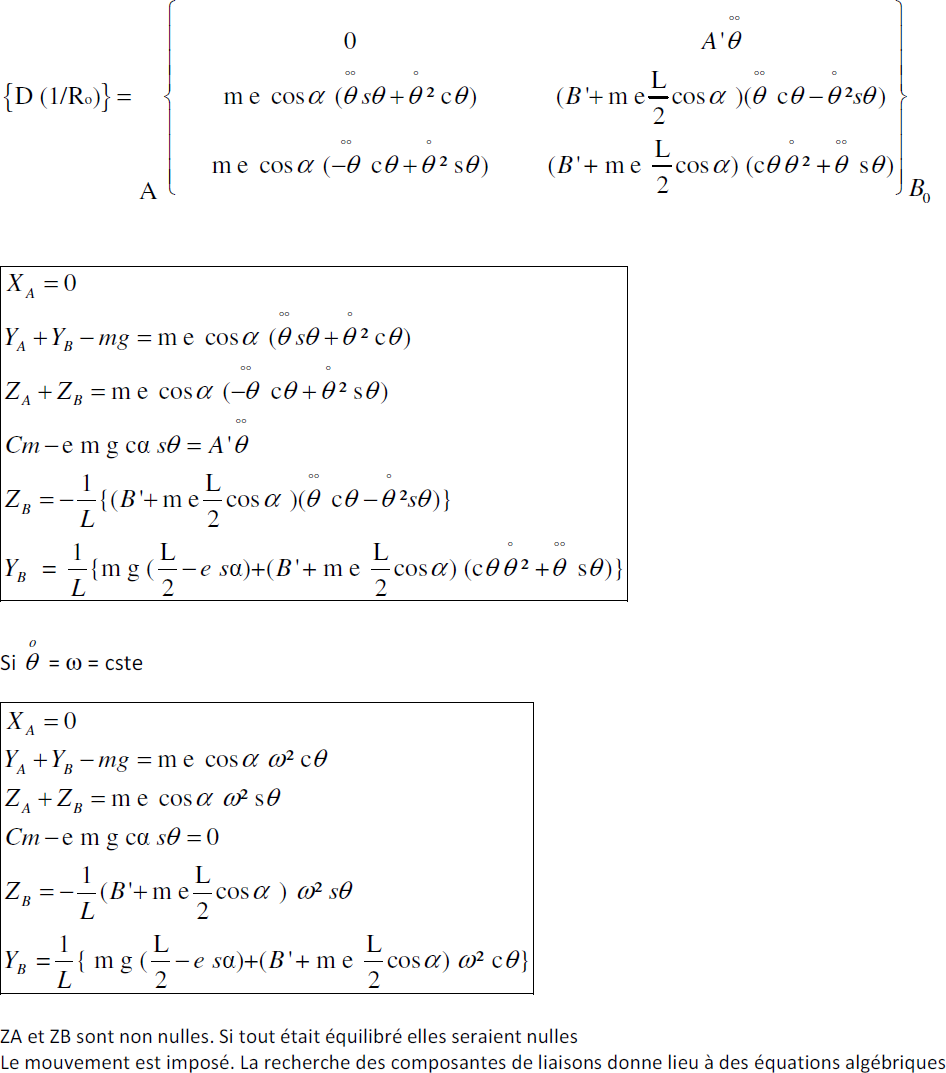
\includegraphics[width=\linewidth]{cor_05}
%\textit{}
\end{center}
\else
\fi

\ifprof
\else
La figure suivante représente l’évolution du couple moteur dans un vérin lors des phases d’ouverture et de fermeture
du coffre.

\begin{center}
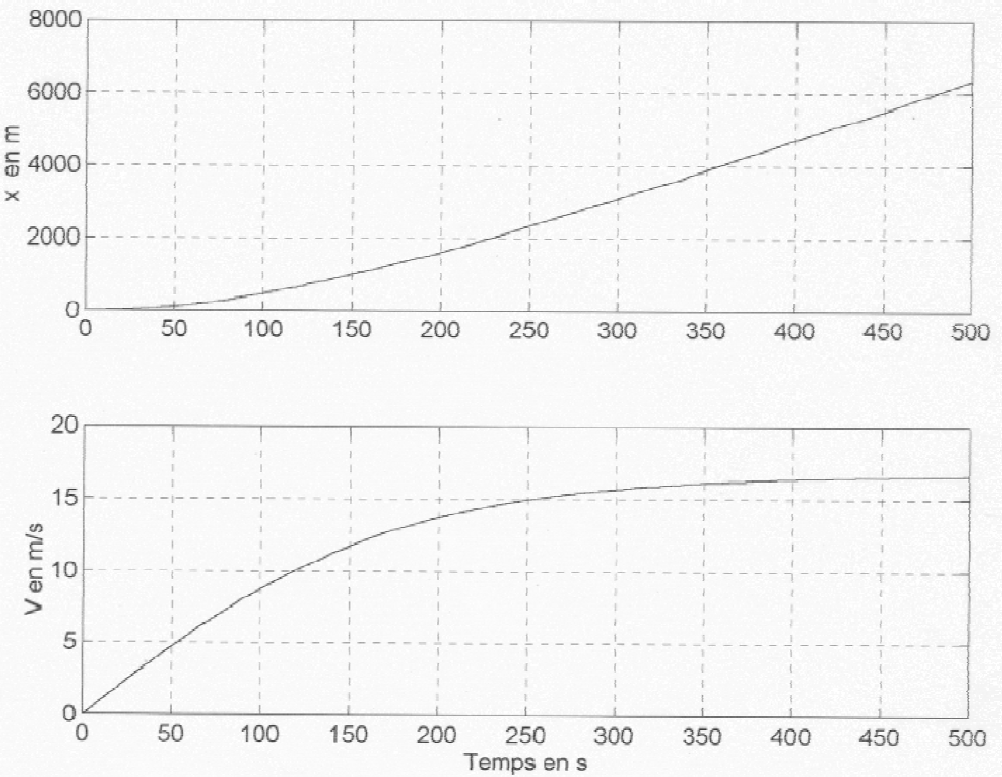
\includegraphics[width=.9\linewidth]{fig_04}
%\textit{}
\end{center}
\fi

\subparagraph{}
\textit{Déterminer le couple moteur maximal en phase d’ouverture puis en phase de fermeture.}
\ifprof
\begin{corrige}~\\
En phase d'ouverture, le couple maximal est de \SI{4e-3}{Nm}. En phase de fermeture il est de \SI{3,5e-3}{Nm}.
\end{corrige}
\else
\fi



\subsection*{Réglage de la fonction sécurité des personnes}

\ifprof
\else
%La commande d’ouverture et de fermeture du coffre est assurée par un asservissement de position angulaire $\theta$
%du hayon. L’étude porte sur l’asservissement d’un seul vérin que nous appellerons « vérin maitre ».
Pour limiter le risque d’accident lié au pincement d’un utilisateur, il est nécessaire de limiter le couple du moteur
à courant continu durant la phase de fermeture du hayon. %Le couple moteur étant proportionnel au courant, il
%faut que la commande du moteur dispose d’un contrôle du courant induit.
%Cette fonction est assurée par une boucle de courant dans la commande du moteur.



On envisage la présence d’un obstacle empêchant la fermeture du coffre. On modélise l’action de l’obstacle sur la porte de coffre par un glisseur s’appliquant en $D$ et s’exprimant $\vect{F_{\text{pinc}}} = F_{\text{pinc}}\vect{y_p}$.

\begin{center}
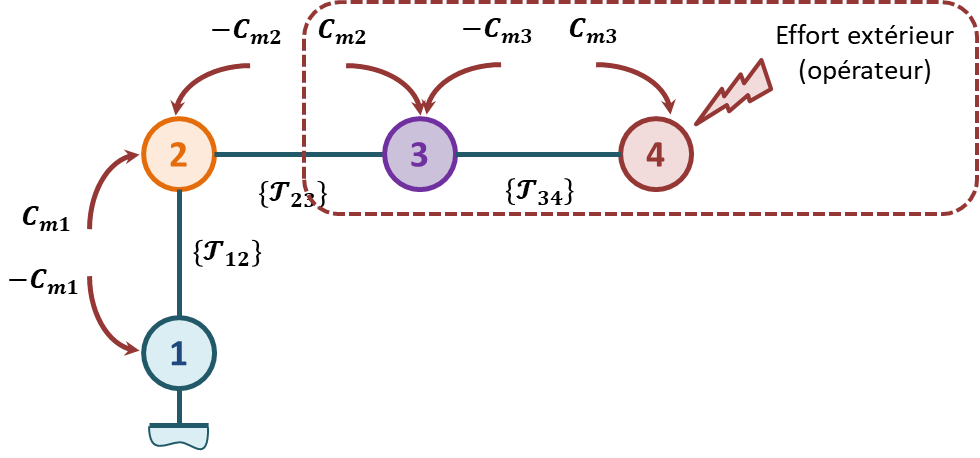
\includegraphics[width=.8\linewidth]{fig_05}
%\textit{}
\end{center}



%\subparagraph{}
%\textit{Quelle doit être la valeur maximale de $ F_{\text{pinc}}$ pour respecter le cahier des charges ?}
%\ifprof
%\begin{corrige}~\\
%
%\end{corrige}
%\else
%\fi

On cherche à déterminer l’accroissement de couple moteur en cas de présence d’obstacle. On suppose ainsi que la
porte de coffre est en équilibre sous l’effet du poids et de l’action des vérins. On ajoute ainsi l’effort de pincement
$ F_{\text{pinc}}$ en $D$ et on cherche l’accroissement d’effort $\Delta F\vec{x}_v$ qu’exercent chacun des vérins en $C$ sur la porte en la supposant en équilibre.

On donne la relation entre le couple moteur et la force fournie par le vérin en régime quasi-statique : $C_m=\rho F$ avec $\rho=\SI{7,89e-5}{m}$.

\fi


\subparagraph{}
\textit{Déterminer l’expression littérale puis la valeur
numérique de $\Delta F$ l’accroissement de la force qu’exerce chacun des vérins sur la porte de hayon.}
\ifprof
\begin{corrige}~\\
On isole le hayon et on réalise le BAME. Le théorème du moment statique en $B$ en projection sur $\vect{z_0}$ : 

$ \left( 
\vect{0} + \vect{BC}\wedge -2\Delta F \vect{x_v}
+ \vect{0} + \vect{BD}\wedge F_{\text{pinc}}\vect{y_0}
\right) \cdot \vect {z_0} = \vect{0} $
$\Rightarrow \left( 
c\vect{x_0}\wedge -2\Delta F \vect{x_v}
+ d\vect{x_0}\wedge F_{\text{pinc}}\vect{y_0}
\right) \cdot \vect {z_0} = \vect{0}$
$\Rightarrow  
-c 2\Delta F  \sin \alpha + dF_{\text{pinc}}  = {0} $
$\Rightarrow  
\Delta F  = \dfrac{dF_{\text{pinc}}}{c 2  \sin \alpha}  $. 

\textit{AN :}
Pour $\theta=0$, $ \tan \alpha = \dfrac{b}{-a+c}=\dfrac{0,14}{-0,55+0,14}=-0,34 \Rightarrow \alpha \simeq -18,8 \degres$.
$\Rightarrow  
\Delta F  = \dfrac{40}{2\cdot 0,14  \sin \alpha} = \SI{-443}{N} $.
\end{corrige}
\else

\fi

La constante de couple du moteur est donnée par $K_t = \SI{9,5e-3}{NmA^{-1}}$.

\subparagraph{}
\textit{En déduire la valeur numérique de l’accroissement $\Delta C_m$  de couple moteur en fonction de la présence d’un obstacle. Déterminer l’intensité maximale du courant dans le moteur lors d’un pincement.}% (on supposera que le rendement de la transmission est unitaire).}
\ifprof
\begin{corrige}~\\
On a $\left|\Delta C_m\right|=\rho \left|\Delta F \right|$ avec $\rho=\SI{7,89e-5}{m}$. En conséquence : $\left|\Delta C_m\right|=443 \cdot 7,89 \cdot 10^{-5} = \SI{35}{mNm}$.

En fin de fermeture, $C_m=\SI{2,5e-3}{Nm}$.
En conséquence $I_{\text{max}}=\dfrac{C_{\text{max}}}{K_t}=\dfrac{C_{m}+\Delta C_m}{K_t}=\dfrac{2,5\cdot 10^{-3}+35\cdot 10^{-3}}{9,5\cdot 10^{-3}}=\SI{3,95}{A}$.

\end{corrige}
\else
\fi

\subsection*{Synthèse}
\subparagraph{}
\textit{Réaliser un poster permettant de synthétiser comment les caractéristiques des composants ont été déterminés.}
%Dans la suite on prendra comme accroissement de couple moteur en cas de pincement une valeur de \SI{0,035}{Nm}. 
%\subparagraph{}
%\textit{}
%\ifprof
%\begin{corrige}~\\
%
%\end{corrige}
%\else
%\fi
\ifprof
\else
\footnotesize
%\vspace{.5cm}

%\begin{multicols}{2}
%%\fbox{
%\noindent Éléments de corrigé 
%\begin{enumerate}
%\item Angle d'ouverture: $67,5\degres$.
%\item $L^2 =\left(-a + c\cos\theta \right)^2 + \left(b + c\sin\theta \right)^2  $.
%\item Course de \SI{13,2}{cm}.
%\item $   F_v = \dfrac{\lambda Mg\cos \theta}{c\sin \left( \alpha - \theta\right)} $ ($F_v/2$).
%\item $k=\SI{1667}{N.m^{-1}}$, écrasement de $\SI{300}{mm}$.
%\item .
%\item $\Delta F = \pm \SI{443}{N}$.
%\item $I_{\text{max}} = \SI{3,95}{A}$.
%\end{enumerate}
%\end{multicols}
\fi

\normalsize


\ifprof
%\end{multicols}
\else
\end{multicols}
\fi

